\documentclass[a4paper, 12pt]{article}
\usepackage{titling}
\usepackage{setspace}
\usepackage{tikz}
\usepackage{algorithm}
\usepackage{graphicx}
\usepackage{subcaption}
\usepackage{listings}
\usepackage[normalem]{ulem}
\usepackage[top=2cm, bottom=1.5cm, left=2cm, right=2cm]{geometry}
\lstset{ %
  language=Python,                     % Le langage utilisé
  basicstyle=\ttfamily\footnotesize, % Style du texte
  keywordstyle=\color{blue},       % Couleur des mots-clés
  commentstyle=\color{teal},      % Couleur des commentaires
  stringstyle=\color{red},         % Couleur des chaînes de caractères
  breaklines=true,                 % Coupure des lignes longues
  numbers=left,                    % Numérotation des lignes
  numberstyle=\tiny\color{gray},   % Style des numéros de ligne
  backgroundcolor=\color{lightgray!20}, % Couleur d'arrière-plan
  frame=single,                    % Encadré autour du code
  captionpos=b                     % Légende en bas du code
}

\title{DM Apprentissage statistique}
\author{Charlotte ARMAND, Lucien DUIGOU}
\date{3 Otobre 2025}

\begin{document}

\begin{flushleft}
    
\includegraphics[width=4cm]{logo.png}
\end{flushleft}

\vspace{2cm}

\begin{center}
    \Huge\textbf{DM Apprentissage statistique} \\[2em]
    \Large Charlotte ARMAND, Lucien DUIGOU \\[1em]
    \large 3 Octobre 2025 
\end{center}

\vspace{3cm}

\begin{center}
    
\includegraphics[width=0.7\textwidth]{photo.png}
\end{center}


\newpage

\tableofcontents
\newpage


\section{Première partie } \label{sec:I}

\subsection{Classification de la classe 1 contre la classe 2 de \textbf{iris}} \label{subsec:classification}


\>\>\>\>\> On se propose d'écrire un code pour classifier la classe 1 contre la classe 2 du dataset \textbf{iris} à l'aide du noyau linéaire et des deux premières variables.

On prend ensuite 75\% des variables pour l'entraînement du modèle (et 25\% en test) et on évalue la performance en généralisation de ce modèle. 

On obtient le code suivant:

\begin{lstlisting}[language=Python, caption=Classification]
iris = datasets.load_iris()
X = iris.data
X = scaler.fit_transform(X)
y = iris.target
X = X[y != 0, :2]
y = y[y != 0]

# split train test
X_train, X_test, y_train, y_test = train_test_split(X, y, test_size=0.25, random_state=0)

# fit the model
parameters = {'kernel': ['linear'], 'C': list(np.logspace(-3, 3, 200))}
clf_linear = SVC()
clf_linear_grid=GridSearchCV(clf_linear, parameters, n_jobs=-1)
clf_linear_grid.fit(X_train, y_train)

# compute the score
print(clf_linear_grid.best_params_)

print('Generalization score for linear kernel: %s, %s' %
      (clf_linear_grid.score(X_train, y_train),
       clf_linear_grid.score(X_test, y_test)))

\end{lstlisting}


\subsection{Comparaison avec un SVM basé sur un noyau polynomial}\label{subsec:comparaison}

On réitère le même procédé avec un noyau polynomial (avec le code suivant). 

\begin{lstlisting}[language=Python, caption=Classification avec noyau polynomial]
Cs = list(np.logspace(-3, 3, 5))
gammas = 10. ** np.arange(1, 2)
degrees = np.r_[2, 3]

parameters = {'kernel': ['poly'], 'C': Cs, 'gamma': gammas, 'degree': degrees}
clf_poly = SVC()
clf_poly_grid=GridSearchCV(clf_poly, parameters, n_jobs=-1)
clf_poly_grid.fit(X_train, y_train)

# compute the score
print(clf_poly_grid.best_params_)

print('Generalization score for polynomial kernel: %s, %s' %
      (clf_poly_grid.score(X_train, y_train),
       clf_poly_grid.score(X_test, y_test)))
\end{lstlisting}

On remarque que le modèle polynomial retient le degré 1, ce qui correspond au modèle linéaire. On fait alors le choix de retirer le degré 1 dans les choix possibles dans le \textit{GridSearch}

\newpage
On trace enfin les frontières obtenues dans les deux cas et on compare les scores. 

\begin{figure}[h!]
    \centering
    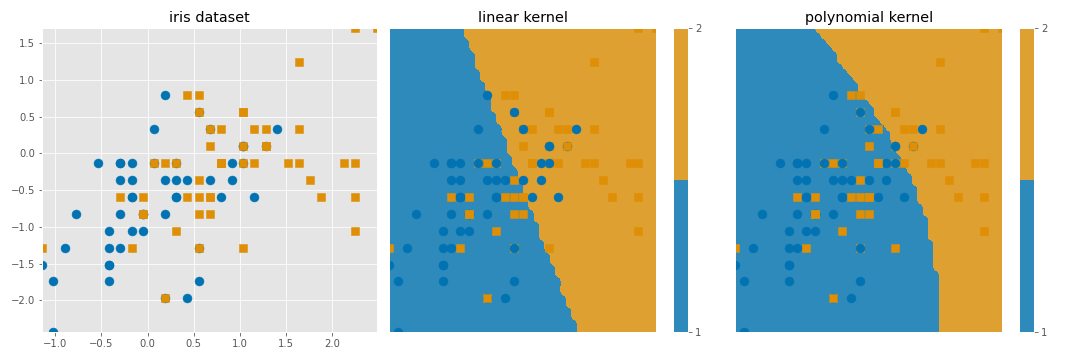
\includegraphics[width=0.9\linewidth]{frontiere_iris.jpeg}
    \caption{Comparaison des frontières en fonction des noyaux choisis}
    \label{fig:ellipses.png}
\end{figure}

On obtient un score pour le noyau linéaire d'environ 0,72 (train) et 0,64 (test). Avec le noyau polynomial, on obtient un moins bon score autour de 0,68 (train) et 0,64 (test). On pouvait s'y attendre vu que le modèle polynomial retient le degré 1 et qu'on lui a imposé de ne pas le prendre. 

A priori, ce modèle est donc moins bon que celui avec un noyau linéaire. 


\newpage
\section{Classification de visages} \label{sec:clavis}

On commence tout d'abord par importer et séparer les données: 
\begin{lstlisting}[language=Python, caption=Importation des données]
# Download the data and unzip; then load it as numpy arrays
lfw_people = fetch_lfw_people(min_faces_per_person=70, resize=0.4,color=True, 
                     funneled=False, slice_=None, download_if_missing=True)

# introspect the images arrays to find the shapes (for plotting)
images = lfw_people.images
n_samples, h, w, n_colors = images.shape

# the label to predict is the id of the person
target_names = lfw_people.target_names.tolist()

names = ['Tony Blair', 'Colin Powell']
idx0 = (lfw_people.target == target_names.index(names[0]))
idx1 = (lfw_people.target == target_names.index(names[1]))
images = np.r_[images[idx0], images[idx1]]
n_samples = images.shape[0]
y = np.r_[np.zeros(np.sum(idx0)), np.ones(np.sum(idx1))].astype(int)

# plot a sample set of the data
plot_gallery(images, np.arange(12))
plt.show()

# Extract features
X = images.copy().reshape(n_samples, -1)

# Scale features
X -= np.mean(X, axis=0)
X /= np.std(X, axis=0)

X_train, X_test, y_train, y_test, images_train, images_test = train_test_split(X, y, images, test_size=0.25, random_state=0)    
\end{lstlisting}

\subsection{Influence du paramètre de régularisation}\label{subsec:influ}

On veut dans cette partie montrer l'influence de \textit{C} (le paramètre de régularisation). Pour cela on représente le score en fonction de \textit{C}. 
On fait cette observation sur une échelle logarithmique. 

On écrit le code permettant de calculer le score de test en fonction des différentes valeurs du paramètre de régularisation \textit{C}. Il choisit ensuite la valeur de \textit{C} qui maximise ce score et construit un modèle utilisant ce paramètre.

\begin{lstlisting}[language=Python, caption=Score du test en fonction de \textit{C}]
    print("--- Linear kernel ---")
print("Fitting the classifier to the training set")
t0 = time()

# fit a classifier (linear) and test all the Cs
Cs = 10. ** np.arange(-5, 6)
scores = []
for C in Cs:
    clf = SVC(kernel='linear',C=C)
    clf.fit(X_train, y_train)
    y_pred = clf.predict(X_test)
    score = clf.score(X_test, y_test)
    scores.append(score)

ind = np.argmax(scores)
print("Best C: {}".format(Cs[ind]))

plt.figure()
plt.plot(Cs, scores)
plt.xlabel("Parametres de regularisation C")
plt.ylabel("Scores d'apprentissage")
plt.xscale("log")
plt.tight_layout()
plt.show()
print("Best score: {}".format(np.max(scores)))

print("Predicting the people names on the testing set")
t0 = time()

# predict labels for the X_test images with the best classifier
clf = SVC(kernel='linear',C=Cs[ind])
clf.fit(X_train, y_train)
y_pred = clf.predict(X_test)

print("done in %0.3fs" % (time() - t0))
# The chance level is the accuracy that will be reached when constantly predicting the majority class.
print("Chance level : %s" % max(np.mean(y), 1. - np.mean(y)))
print("Accuracy : %s" % clf.score(X_test, y_test))
\end{lstlisting}

On obtient l'évolution du score en fonction du paramètre. 
On le représente comme suit: 

\begin{figure}[h!]
    \centering
    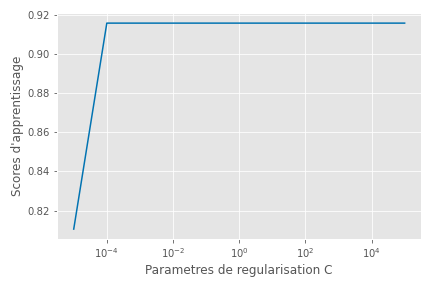
\includegraphics[width=0.7\linewidth]{evolution_score.png}
    \caption{Evolution du score}
    \label{fig:placeholder}
\end{figure}

En observant ce graphique, on voit que le score de test atteint son maximum et reste constant à partir de \textit{C}=0.0001 le modèle retenu est donc celui avec \textit{C}=0.0001. Son score de test est d'environ 0.916.

Après avoir entraîné le modèle pour cette valeur de \textit{C}, le code nous indique une "Chance level" d'environ 62\%, c'est-à-dire que sur les données test, le modèle fait une bonne prédiction dans 62\% des cas. 

Voici un exemple de prédiction de test avec le nom prédit et le vrai nom. Dans cette portion de test, le modèle a eu raison à chaque fois. 

Enfin, on trace le graphe des coefficients du prédicteur évalués en trichromie.
\begin{figure}[H]

  \begin{minipage}{0.45\linewidth}
   \centering
   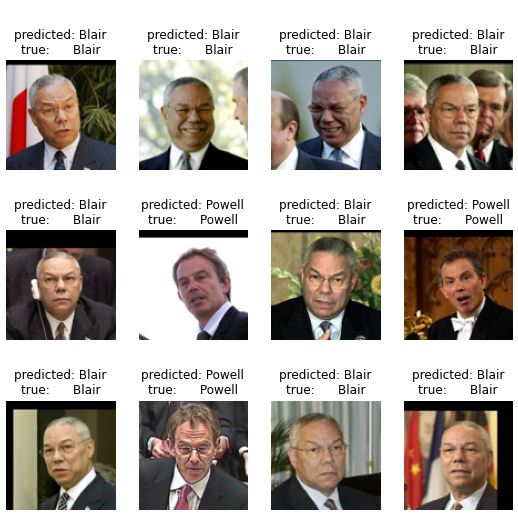
\includegraphics[width=9cm,height=9cm]{prediction_test.png}
   \caption{Prédiction de test}
  \end{minipage}
    \hfill
  \begin{minipage}{0.45\linewidth}
   \centering
   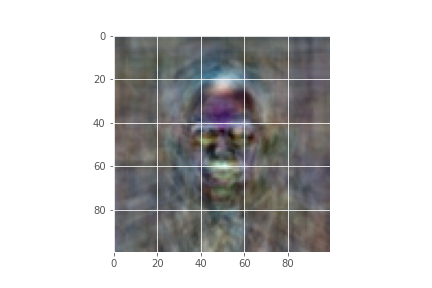
\includegraphics[trim = 3cm 0cm 3.5cm 1cm, clip]{graph_coef.png}   
   \caption{Coefficients du prédicteur}
  \end{minipage}
  \label{fig:ma_fig}
\end{figure}


\subsection{Influence du nombre de variance}\label{subsec:influvar}

On choisit ensuite d'ajouter des variables de nuisance. On observe alors leur influence sur la performance. 

Le code suivant mesure les valeurs du score avant puis après ajout de nuisance (3\% de bruit). 

\begin{lstlisting}[language=Python, caption=Calcul des scores avant et après nuisance]
def run_svm_cv(_X, _y):
    _indices = np.random.permutation(_X.shape[0])
    _train_idx, _test_idx = _indices[:_X.shape[0]//2], _indices[_X.shape[0]//2:]
    _X_train, _X_test = _X[_train_idx, :], _X[_test_idx, :]
    _y_train, _y_test = _y[_train_idx], _y[_test_idx]
    _parameters = {'kernel': ['linear'], 'C': list(np.logspace(-3, 3, 5))}
    _svr = svm.SVC()
    _clf_linear = GridSearchCV(_svr, _parameters)
    _clf_linear.fit(_X_train, _y_train)
    print('Generalization score for linear kernel: %s, %s \n' %
            (_clf_linear.score(_X_train, _y_train), _clf_linear.score(_X_test, _y_test)))
            
print("Score sans variable de nuisance")
run_svm_cv(X,y)
print("Score avec variable de nuisance")
n_features = X.shape[1]
sigma = 1
noise = sigma * np.random.randn(n_samples, 900, )
indice=np.random.permutation(X.shape[1])
indice=[indice[i] for i in range(0,900)]
X_new=np.delete(X,indice, axis=1)
indice2=np.random.permutation(X_new.shape[1])
X_new=X[:,indice2]
X_noisy=np.concatenate((X_new,noise), axis=1)
run_svm_cv(X_noisy, y)
\end{lstlisting}
Avant nuisance, on obtient les scores : 1.0 (train) et 0.926 (test)\\
Après nuisance : 1 (train) et 0.895 (test)

On voit bien que la performance sur les données de test chute avec l'augmentation du nombre de variables bruitées (environ 1\%).

\subsection{Réduction de dimension}\label{subsec:reduction}

En tenant compte des conclusions des parties précédentes, on choisit de réduire la dimension.

\begin{lstlisting}[language=Python, caption= réduction de dimension]
print(" Evolution du score en fonction de la dimension")
n_components = [10*i for i in range(1,38)] # jouer avec ce parametre

scores=[]
for i in n_components:
    pca = PCA(n_components=i).fit(X_noisy)
    score=float(run_svm_cv(pca.transform(X_noisy), y).split(':')[1].split(' ')[2])
    scores.append(score)

plt.figure()
plt.plot(n_components, scores)
plt.xlabel("nombre de composantes")
plt.ylabel("Scores d'apprentissage")
plt.tight_layout()
plt.draw()

ind=np.argmax(scores)
print('Nombre de composantes retenues :',n_components[ind])
print('Score maximum atteint :',scores[ind])
\end{lstlisting}

Au regard de ce que nous renvoie le code ci-dessus, le graphique montrant l'évolution du score de test selon le nombre de composantes retenues nous informe sur l'influence de ce di nombre dans la performance du modèle. 

Dans notre cas, on peut supposer que la dimension 230 est celle qui ajuste au mieux le modèle avec un score d'environ 0.942.

\begin{figure}[h!]
    \centering
    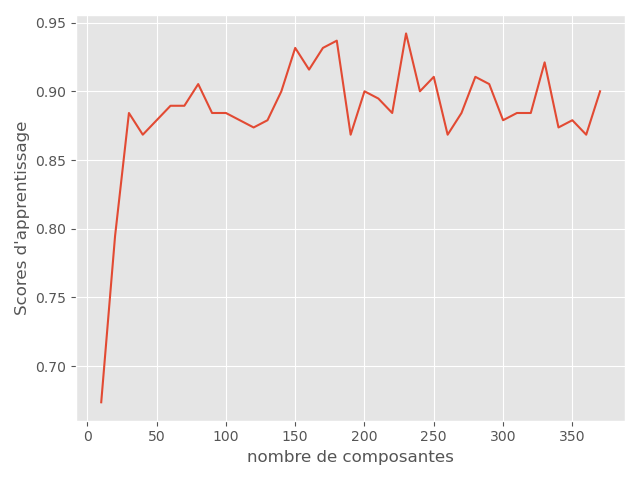
\includegraphics[width=0.67\linewidth]{score_reduction.png}
    \caption{Evolution du score selon la dimension}
    \label{fig:placeholder}
\end{figure}

\newpage

\subsection{Recherche du biais}

On remarque un biais dès le prétraitement de nos données. 

En effet, on fait un choix aléatoire de séparation de données d’entraînement et de test avec 25\% des données totales en test, puis on entraîne notre modèle en maximisant le score de test. 

L’idéal serait de faire ce travail pour toutes les façons de séparer les données et de prendre le meilleur modèle parmi tous les modèles sélectionnés. 


\end{document}
